\section{Explicit $\hat\zeta$ calculation for $P_1=-1$}
\label{app:explicit_zeta}
Setting the right-hand side of Eq. \eqref{constraints} to zero implies that the bracketed term
\begin{equation*}
\left[\frac{P_{1}}{m_{N}}\left(\hat{\zeta}-\sqrt{\hat{\zeta}^2+1}\right)+\hat{\zeta}\frac{m_{N}}{P_{1}}\right]
\end{equation*}
must vanish. This fixes the required Collins-Soper parameter, up to a sign, for a given lattice momentum. Using the lattice ensemble parameters from our lattice size of $\{\hat{L}^3\times\hat{T}\}=\{32^3\times96\}$ and lattice unit of $a=0.11403\text{ fm}$ (pion mass $m_\pi=317\text{ MeV}$), the nucleon mass and the lowest momentum mode are:
\begin{align}
    \mN &= \frac{0.6228(28)}{0.11403\text{ fm}} =  \frac{0.6228(28)\times 197.32698 \text{ MeV}}{0.11403} = 1077.8(48)\text{ MeV} \ , \\
    P_{1}&=-\frac{2\pi}{L}=-\frac{2\pi}{32\times 0.11403\text{ fm}}=-339.8\text{ MeV} \ .
\end{align}
Substituting these values into the constraint equation yields:
\begin{align}
   \Longrightarrow \left[\frac{P_{1}}{m_{N}}\left(\hat{\zeta}-\sqrt{\hat{\zeta}^2+1}\right)+\hat{\zeta}\frac{m_{N}}{P_{1}}\right]&=0 \nonumber \\
    \Longrightarrow \hat{\zeta} &=\sqrt{\frac{P_{1}^2}{m_{N}^{2}\left(\frac{m_{N}^{2}}{P_{1}^{2}}+2\right)}} \nonumber \\
    \hat{\zeta} &= \pm 0.09077(75) \nonumber \\
    \Aboxed{\hat{\zeta} &= \pm 0.090772} \ .
\end{align}
With $\hat{\zeta}$ determined, we can derive the specific orientation of the space-like staple vector $v$. From the definition of $\hat{\zeta}$:
\begin{align}
    \hat{\zeta}&=\frac{-v_{1}P_{1}}{|v|\mN}=\frac{-v_{1}P_{1}}{\left(\sqrt{v_{1}^{2}+0^{2}+v_{3}^{2}}\right)m_{N}} \ .
\end{align}
Solving for the longitudinal staple component $v_1$ in terms of the transverse component $v_3$:
\begin{align}
    \Longrightarrow\Aboxed{v_{1}=\pm 0.301~v_{3}} \ .
\end{align}

The same calculation for $P_1=-2,-3,-4$ gives the values in Table~\ref{tab:zeta_directions}.

\section{Gauge-link paths}
\label{app:paths}
\subsection{Staple paths}
\begin{figure}[htpb]
    \centering
    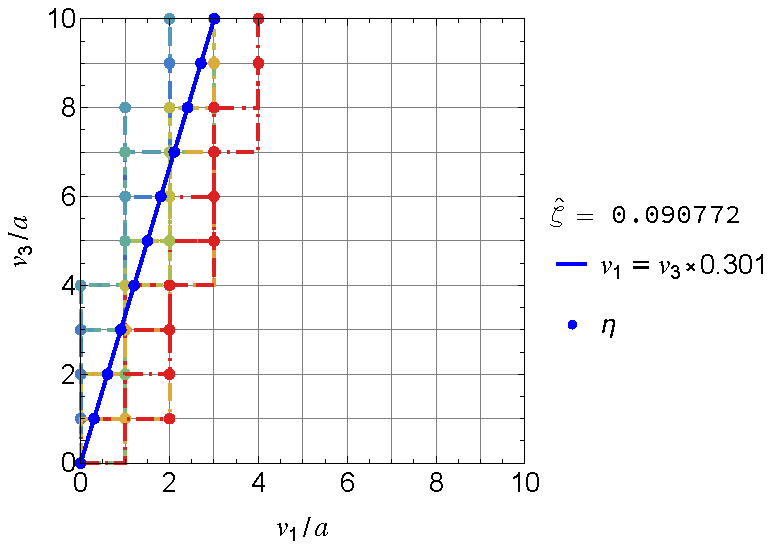
\includegraphics[width=0.6\linewidth]{figures/v1_v2_withPath_forP-1_plot.pdf}
        \caption{Ideal continuous trajectory of the off-axis staple vector (solid blue) for $P_1 = -1$. Circular markers indicate target continuous coordinates for sequential values of $\eta$. Dashed lines illustrate the discrete, step-wise permutations of gauge links used to reach the surrounding bounding integer lattice sites.}
        \label{fig:v_path_P-1}
\end{figure}

\begin{table*}[htbp]
    \centering
    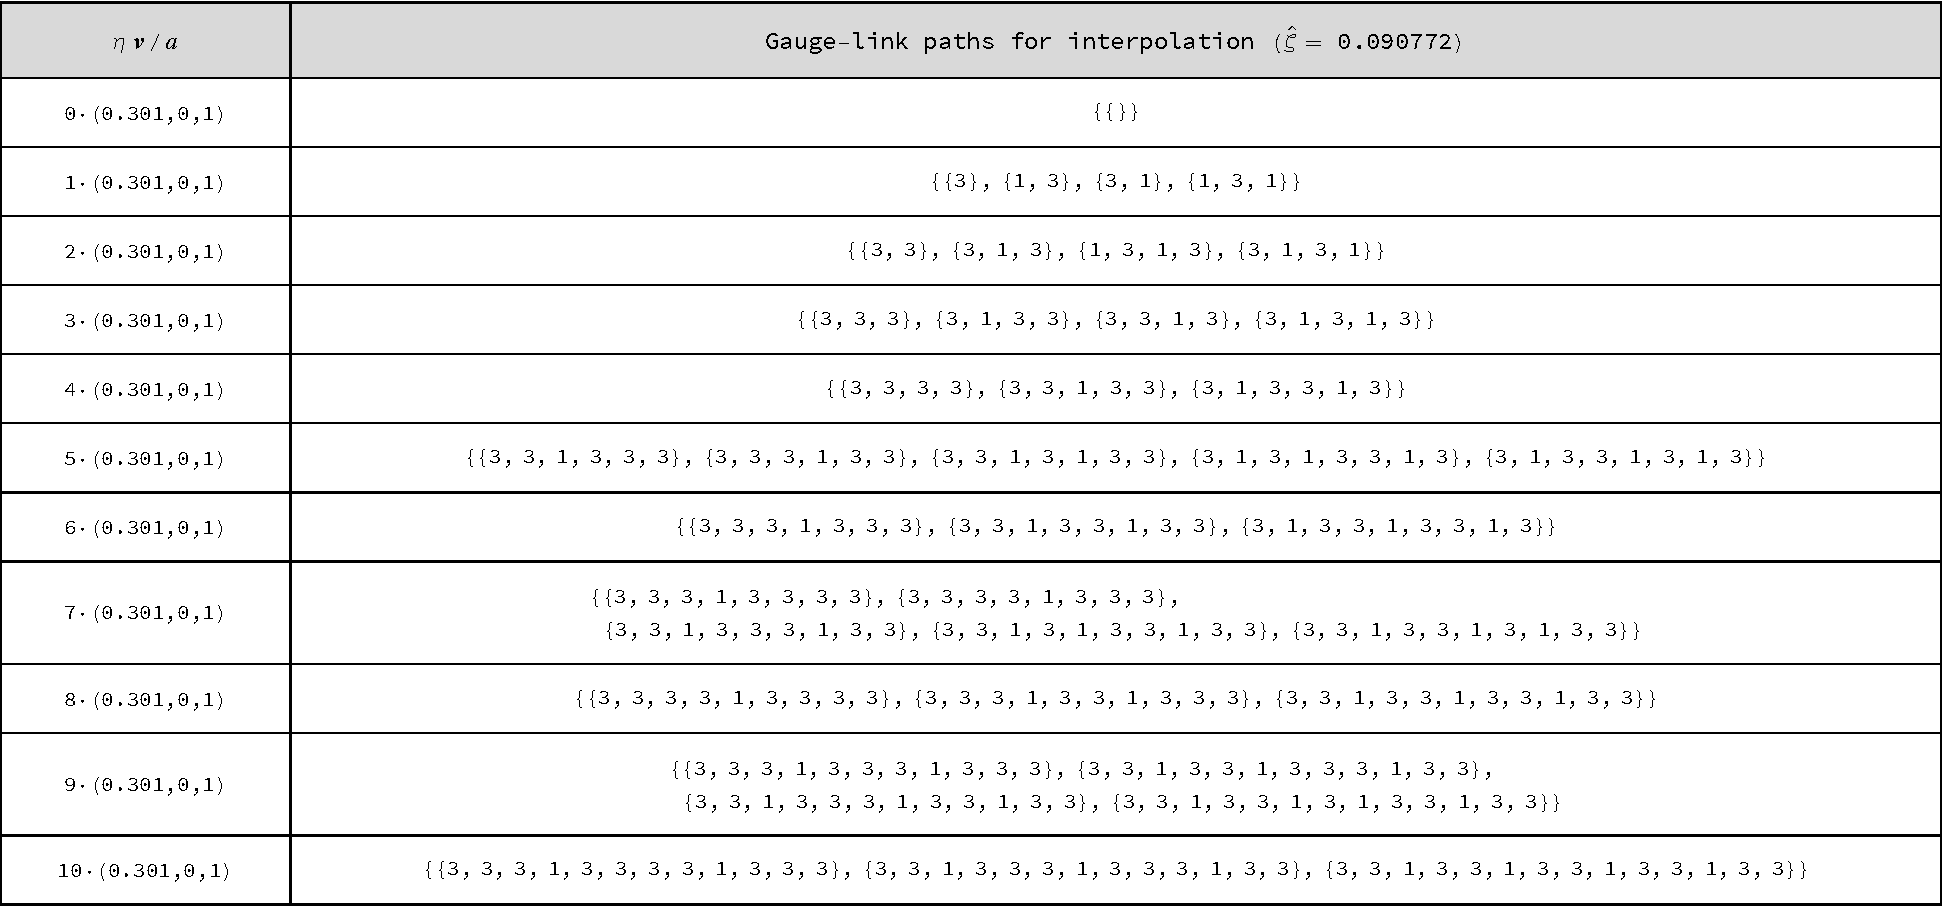
\includegraphics[width=0.8\textwidth,height=0.45\textheight,keepaspectratio]{figures/eta_gauge_links_forP-1_table.pdf}
        \caption{Discrete gauge link configurations defining the interpolation bounds for $P_1 = -1$. Empty brackets $\{\}$ denote a zero-length origin link, while numerical arrays (e.g., $\{1,3,1\}$) give the sequence of directional steps.}
        \label{tab:eta_table_P-1}
\end{table*}


% ---------------------------------------------------------
% P_1 = -2 Figures
% ---------------------------------------------------------
\begin{figure}[htpb]
    \centering
    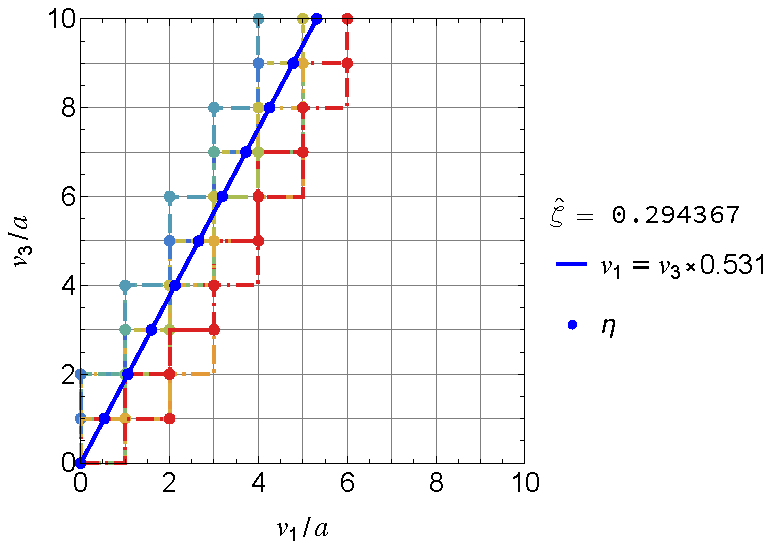
\includegraphics[width=0.6\linewidth]{figures/v1_v2_withPath_forP-2_plot.pdf}
        \caption{Ideal continuous trajectory and corresponding discrete bounding paths for the off-axis staple vector at $P_1 = -2$.}
        \label{fig:v_path_P-2}
\end{figure}

\begin{table*}[htbp]
    \centering
    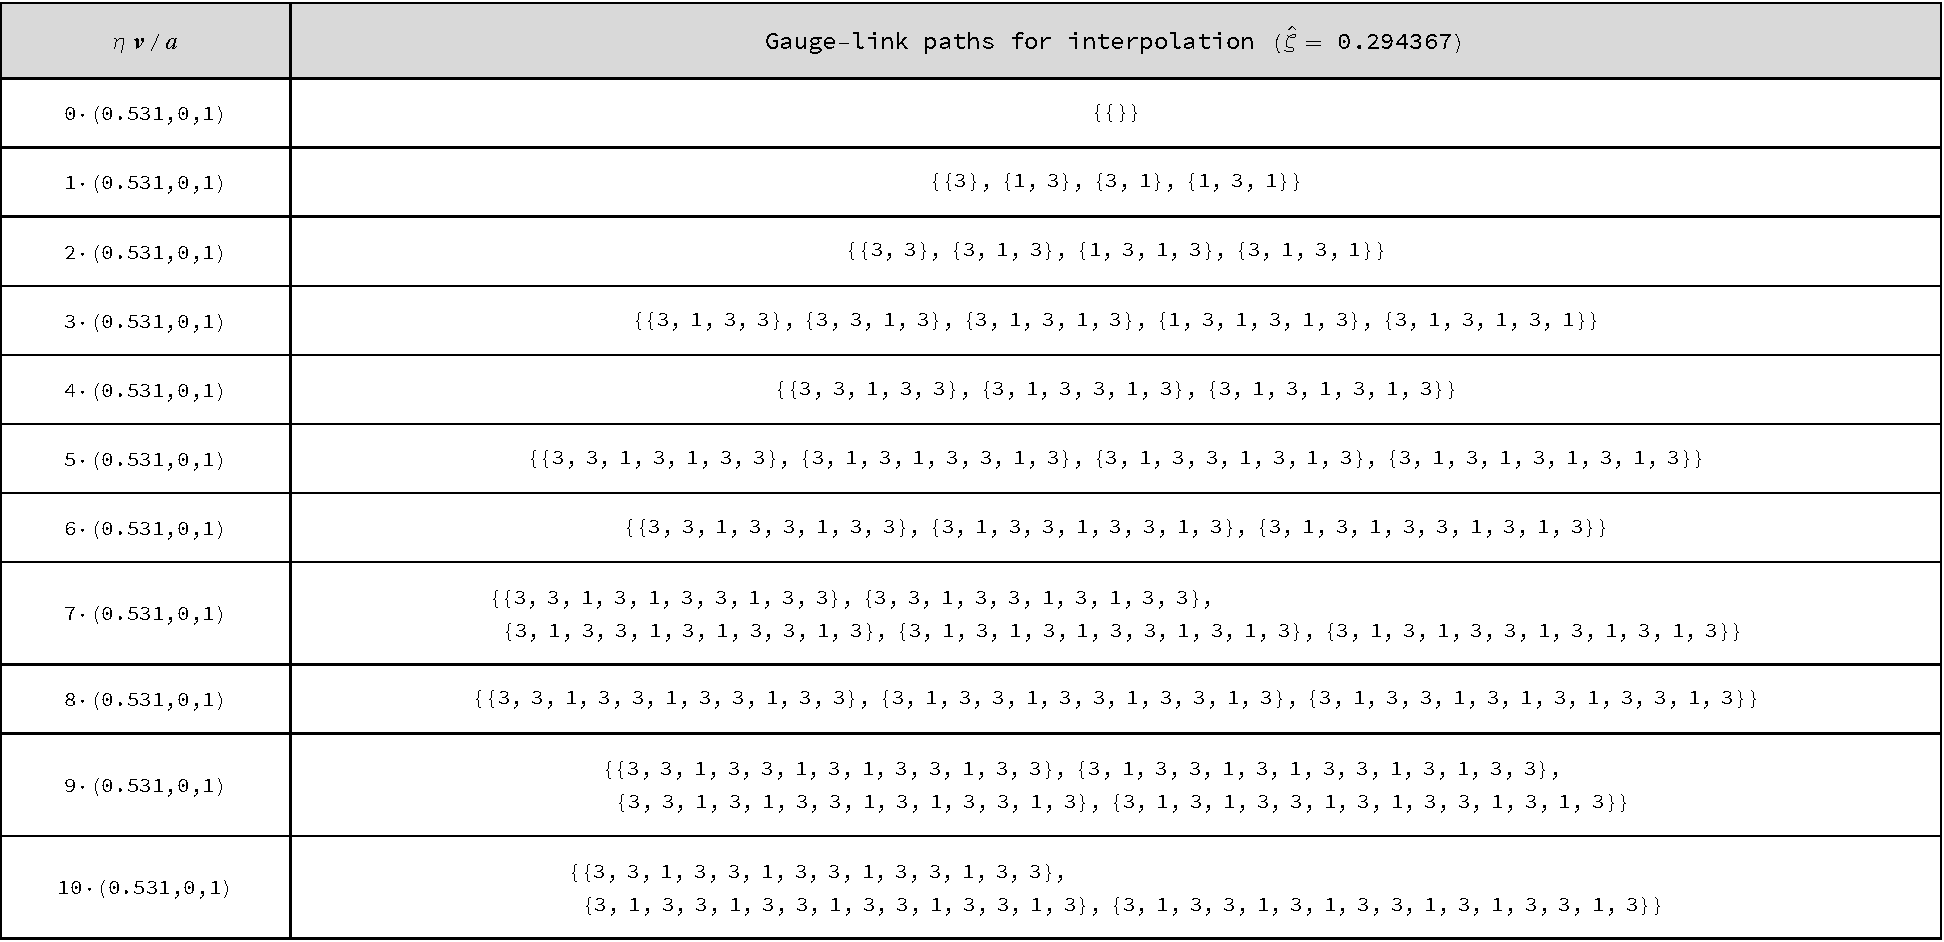
\includegraphics[width=0.8\textwidth,height=0.45\textheight,keepaspectratio]{figures/eta_gauge_links_forP-2_table.pdf}
        \caption{Discrete gauge link configurations defining the interpolation bounds for $P_1 = -2$.}
        \label{tab:eta_table_P-2}
\end{table*}


% ---------------------------------------------------------
% P_1 = -3 Figures
% ---------------------------------------------------------
\begin{figure}[htpb]
    \centering
    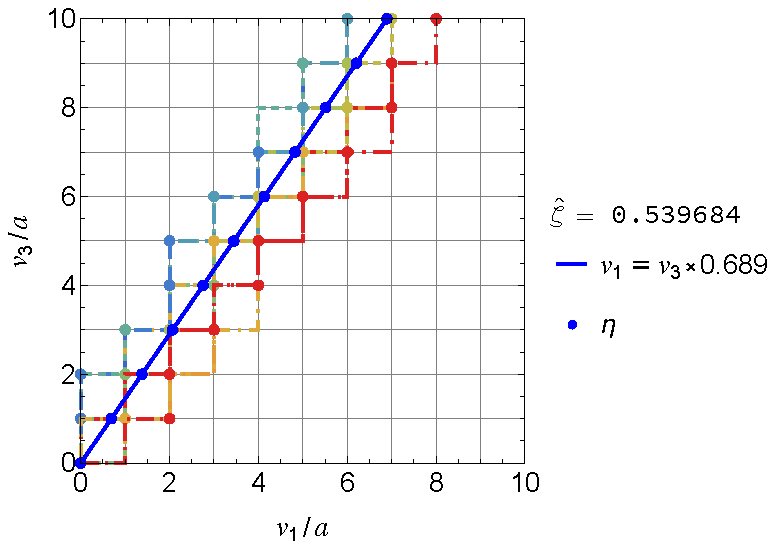
\includegraphics[width=0.6\linewidth]{figures/v1_v2_withPath_forP-3_plot.pdf}
        \caption{Ideal continuous trajectory and corresponding discrete bounding paths for the off-axis staple vector at $P_1 = -3$.}
        \label{fig:v_path_P-3}
\end{figure}

\begin{table*}[htbp]
    \centering
    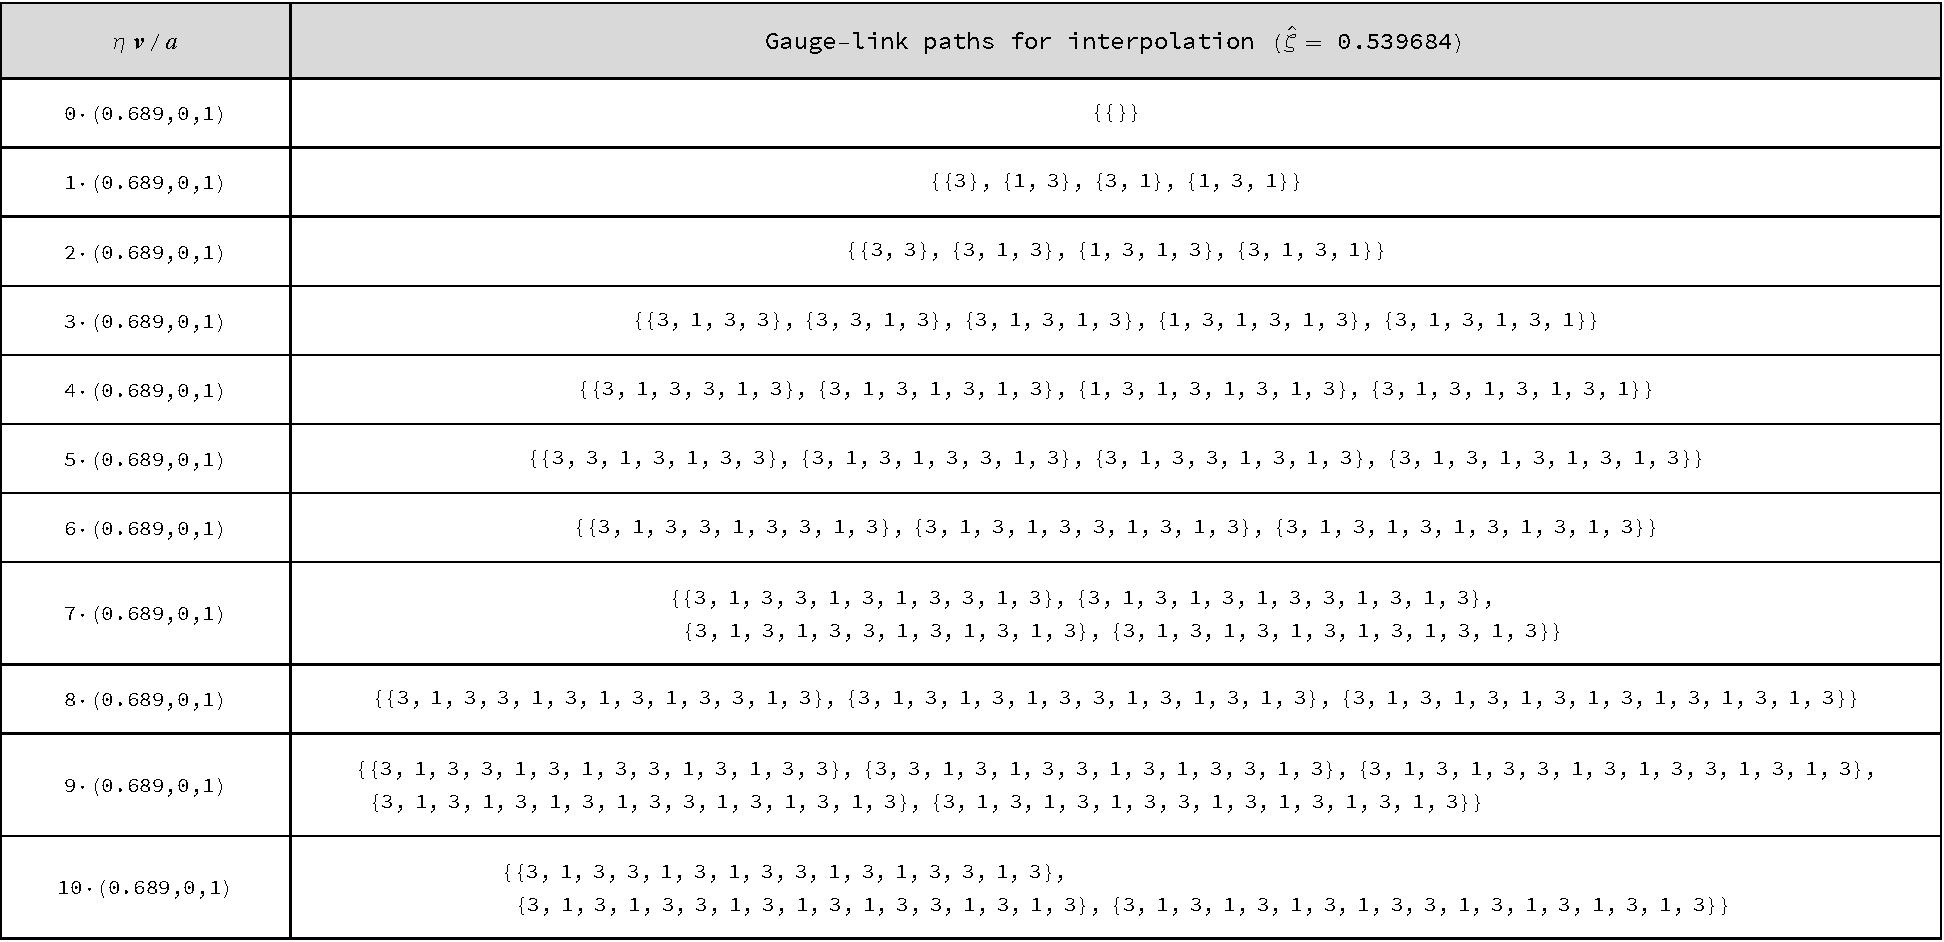
\includegraphics[width=0.8\textwidth,height=0.45\textheight,keepaspectratio]{figures/eta_gauge_links_forP-3_table.pdf}
        \caption{Discrete gauge link configurations defining the interpolation bounds for $P_1 = -3$.}
        \label{tab:eta_table_P-3}
\end{table*}


% ---------------------------------------------------------
% P_1 = -4 Figures
% ---------------------------------------------------------
\begin{figure}[htpb]
    \centering
    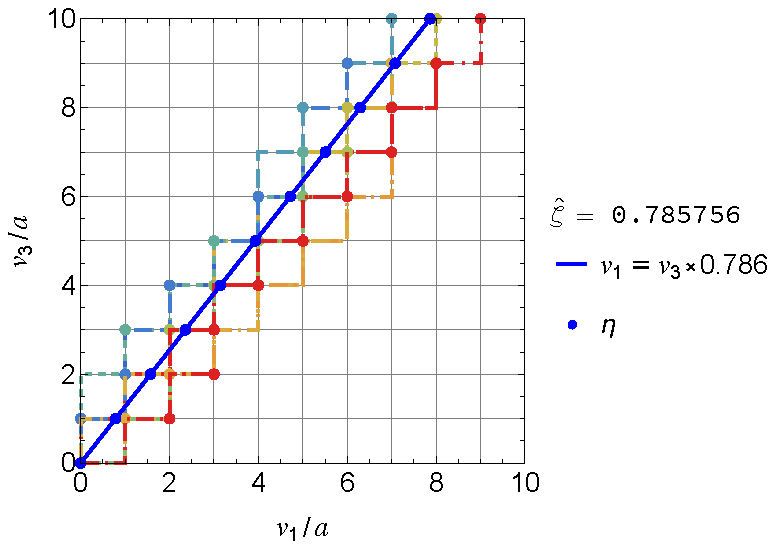
\includegraphics[width=0.6\linewidth]{figures/v1_v2_withPath_forP-4_plot.pdf}
        \caption{Ideal continuous trajectory and corresponding discrete bounding paths for the off-axis staple vector at $P_1 = -4$.}
        \label{fig:v_path_P-4}
\end{figure}

\begin{table*}[htbp]
    \centering
    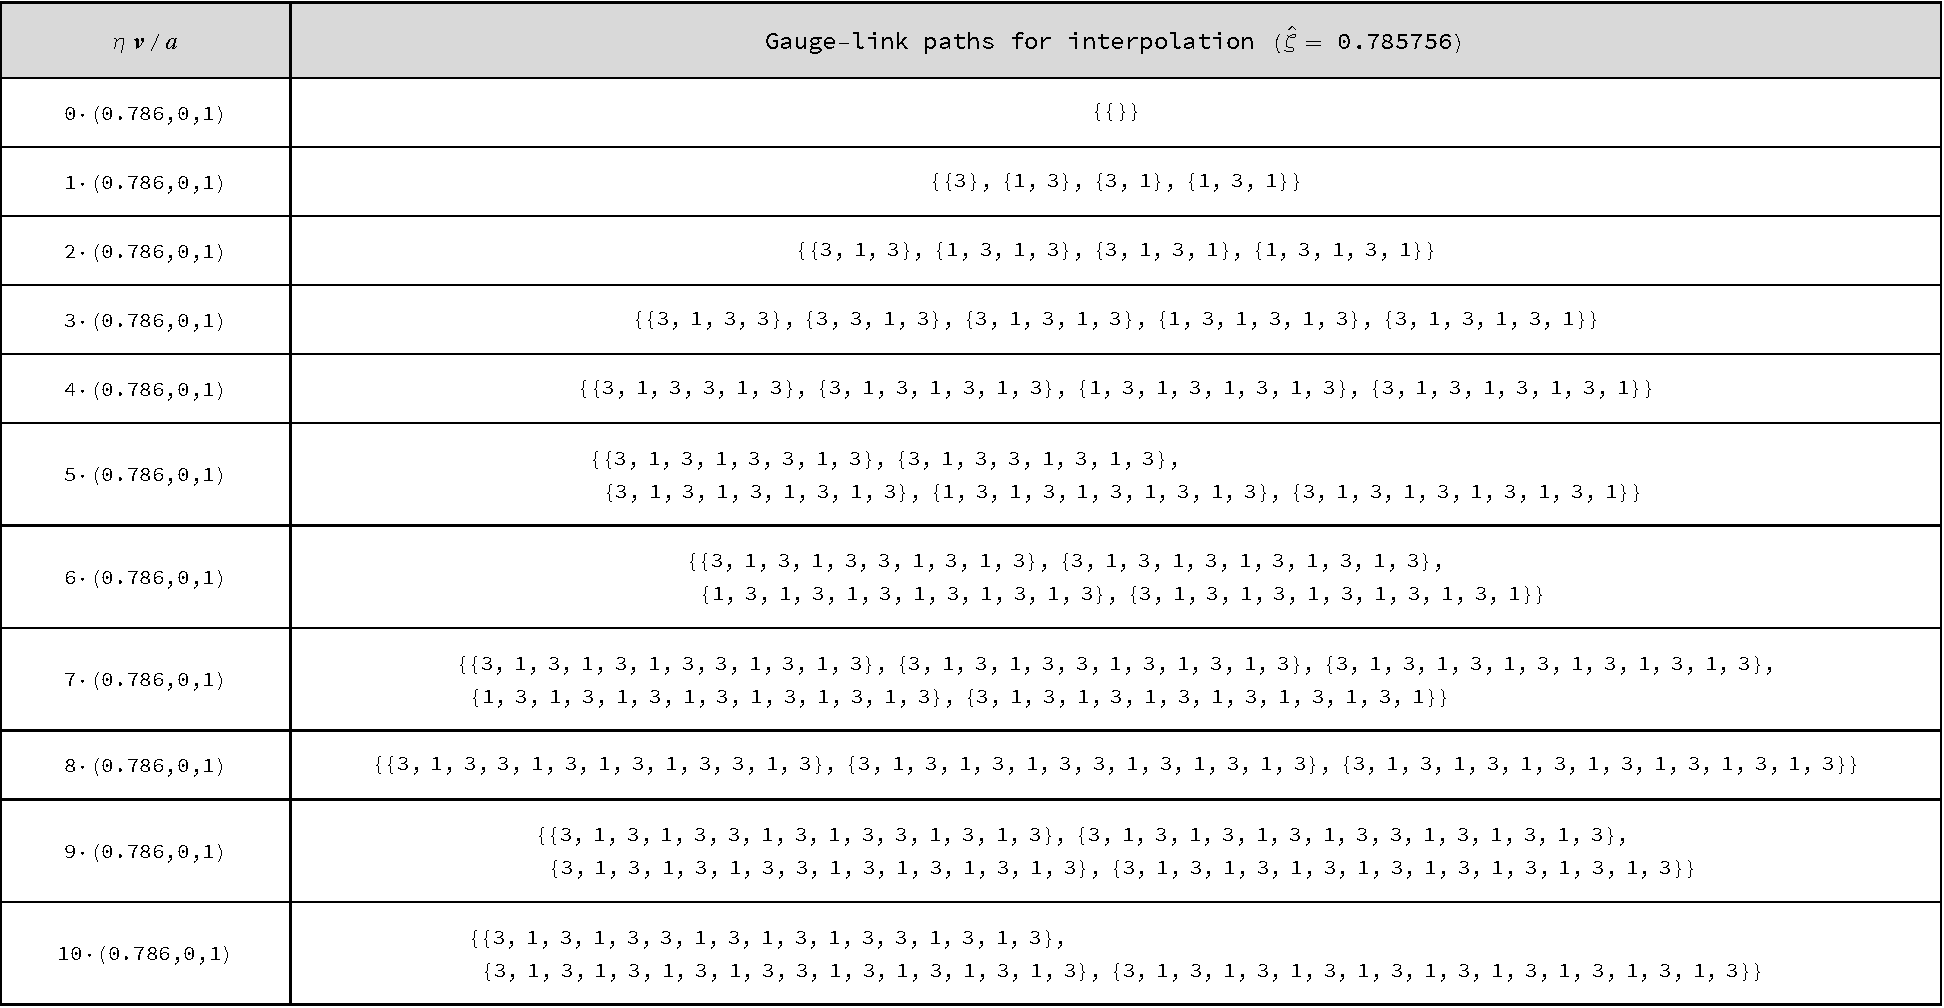
\includegraphics[width=0.8\textwidth,height=0.45\textheight,keepaspectratio]{figures/eta_gauge_links_forP-4_table.pdf}
        \caption{Discrete gauge link configurations defining the interpolation bounds for $P_1 = -4$.}
        \label{tab:eta_table_P-4}
\end{table*}

\subsection{Paths for the quark separation \texorpdfstring{$\vect{b}$}{b}}
\label{sec:b_gauge_links}
Constructing the direct Wilson line connecting the quark fields at $0$ and $\vect{b}$ requires generating step-wise paths across the lattice. We categorize these paths into purely transverse separations ($b_1 = 0$) and off-axis separations with a longitudinal component ($b_1 \neq 0$). For purely transverse separations, where $b \cdot P = 0$, the gauge links lie entirely within the transverse plane. Table \ref{tab:b_table_transverse} lists the link sequences used to reach these target coordinates. An empty bracket $\{\}$ denotes the local origin, while arrays such as $\{2,2\}$ indicate a sequence of two consecutive links in the $\hat{x_{2}}$-direction.

\begin{table*}[htbp]
    \centering
    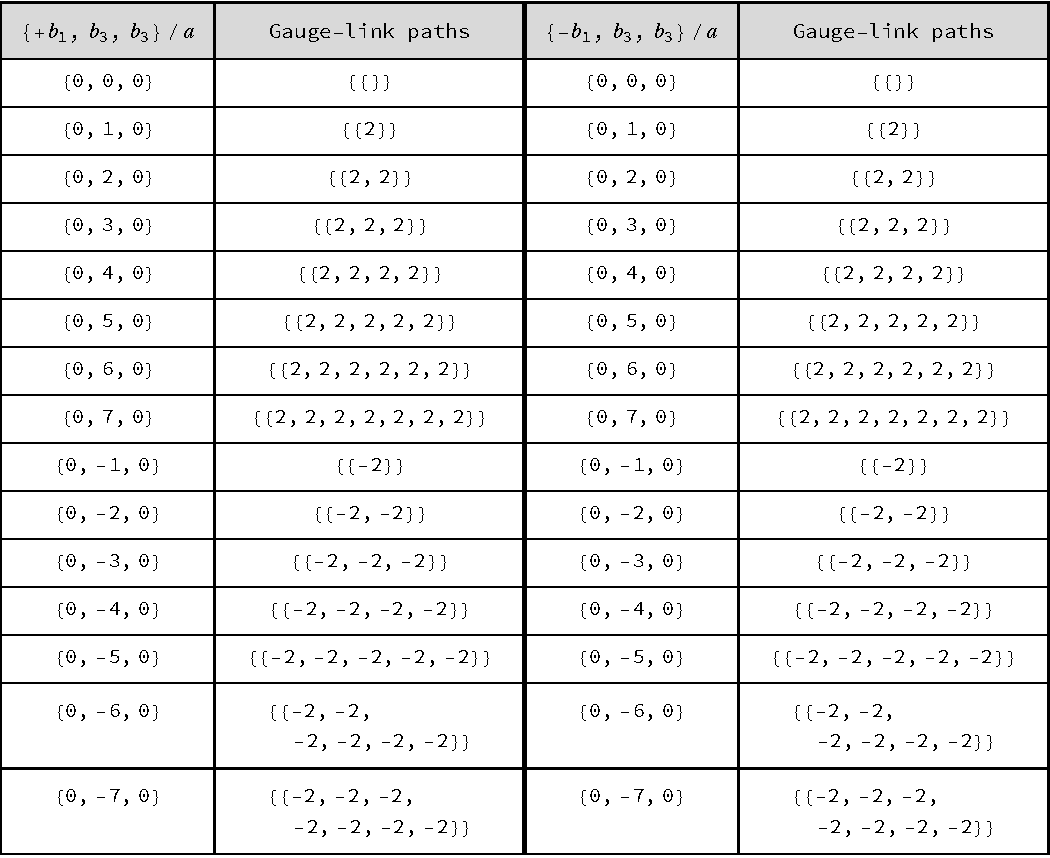
\includegraphics[width=0.8\textwidth,height=0.45\textheight,keepaspectratio]{figures/b_gauge_links_for_table1.pdf}
    \caption{Discrete gauge link configurations for purely transverse quark separations ($\vect{b} = \{0, b_2, 0\}$). The numerical arrays show the sequential lattice steps (e.g., `2` represents a shift in the $x_2$ direction). Our lattice size is $\{\hat{L}^3\times\hat{T}\}=\{32^3\times96\}$ and the lattice spacing is $a=0.11403\text{ fm}$.}
    \label{tab:b_table_transverse}
\end{table*}

To access finite $b \cdot P$, we construct off-axis paths with simultaneous steps in the longitudinal ($\hat{x_{1}}$) and transverse ($\hat{x_{2}}$) directions. To preserve the symmetry required for isolating parity states, every path that reaches a $+b_1$ coordinate has an exact mirror path reaching $-b_1$. Tables \ref{tab:b_table_pos_b1}-\ref{tab:b_table_neg_b1} show these mirrored sequences side by side. Sequences such as $\{2,1\}$ indicate an alternating ``staircase'' step: one unit in the $\hat{x_{2}}$-direction followed by one unit in the $\hat{x_{1}}$-direction. 
\begin{table*}[htbp]
    \centering
    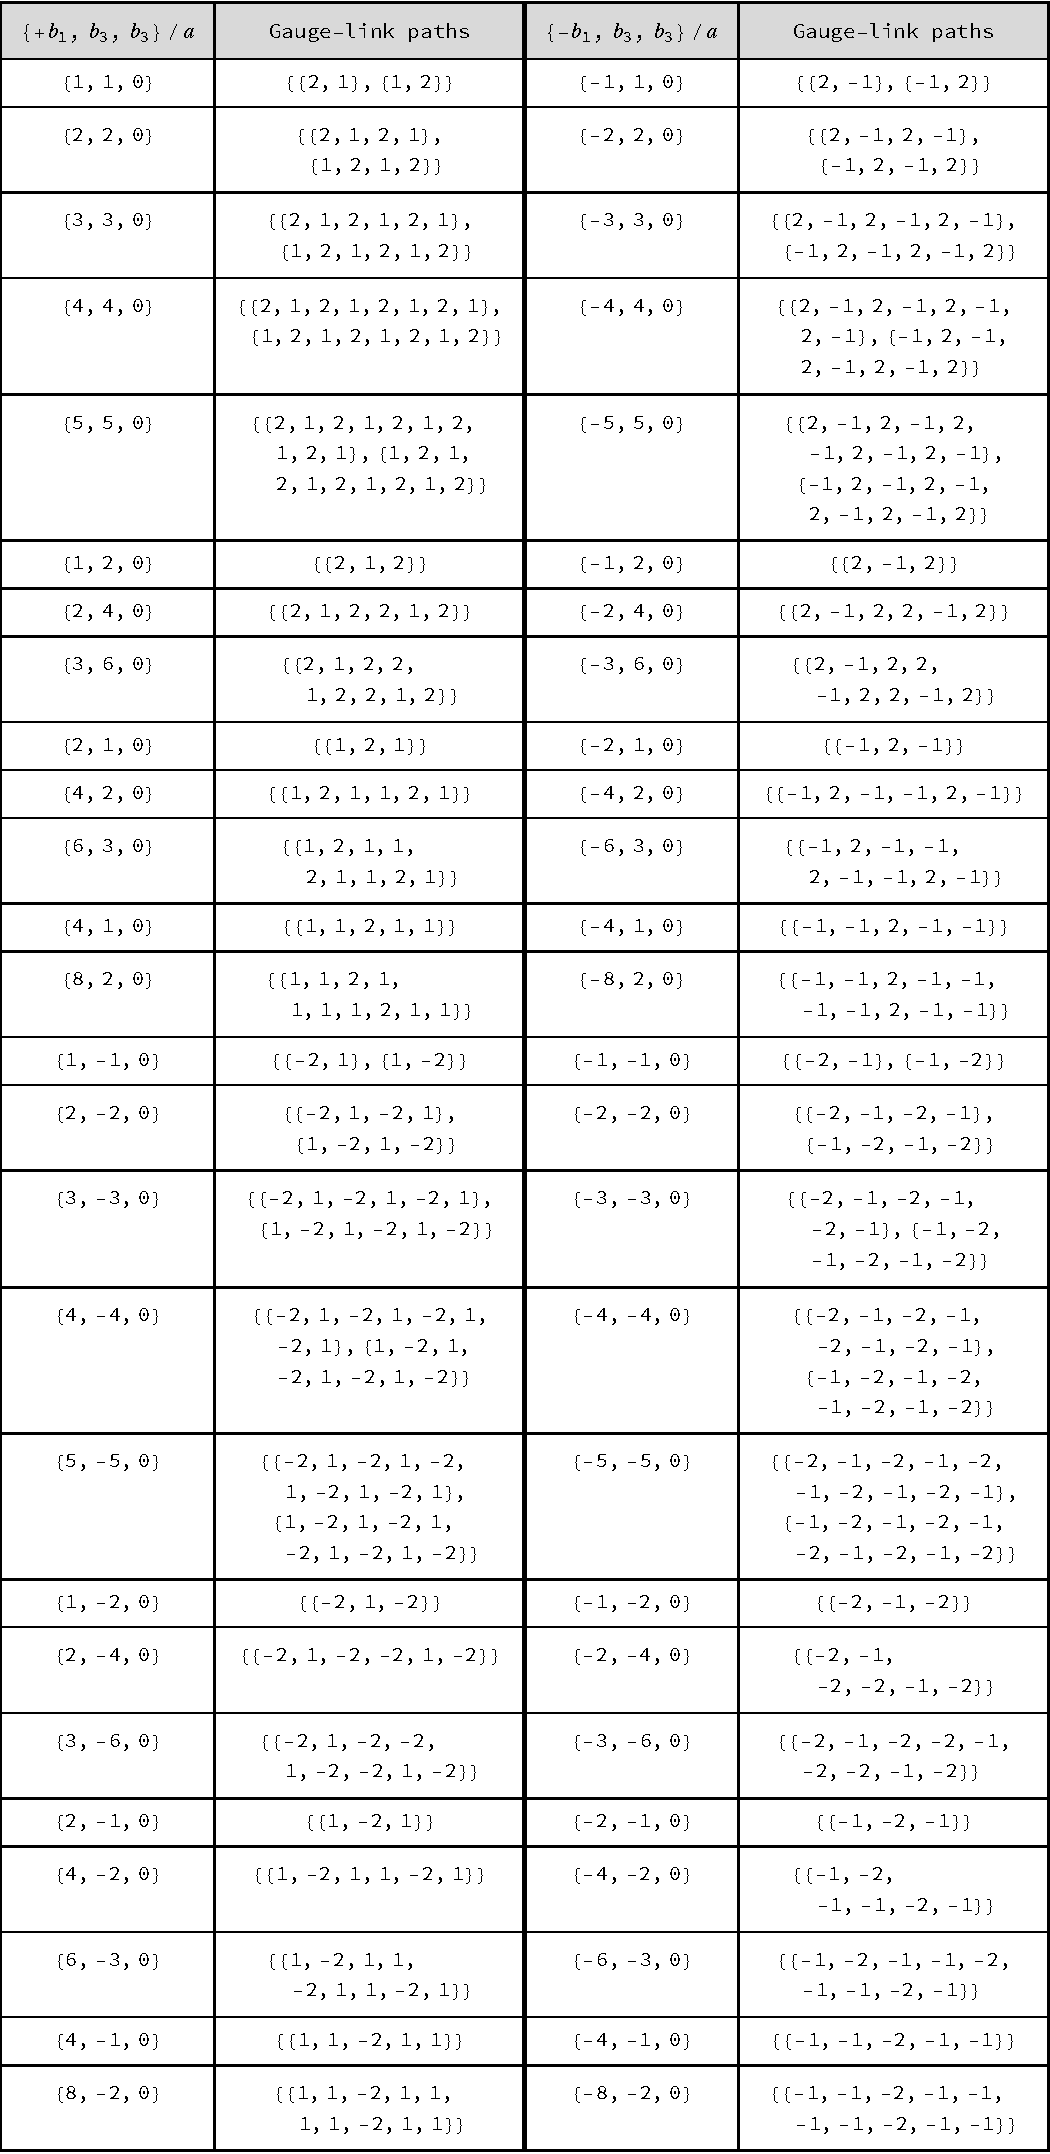
\includegraphics[width=0.8\textwidth,height=0.45\textheight,keepaspectratio]{figures/b_gauge_links_for_table2.pdf}
        \caption{Gauge link sequences for $+b_1$ (positive longitudinal separation). Symmetric sets of step-wise gauge link paths required to access finite $\pm b \cdot P$ and isolate the real and imaginary components of the invariant amplitudes. Our lattice size is $\{\hat{L}^3\times\hat{T}\}=\{32^3\times96\}$ and the lattice spacing is $a=0.11403\text{ fm}$.}
        \label{tab:b_table_pos_b1}
\end{table*}

\begin{table*}[htbp]
    \centering
    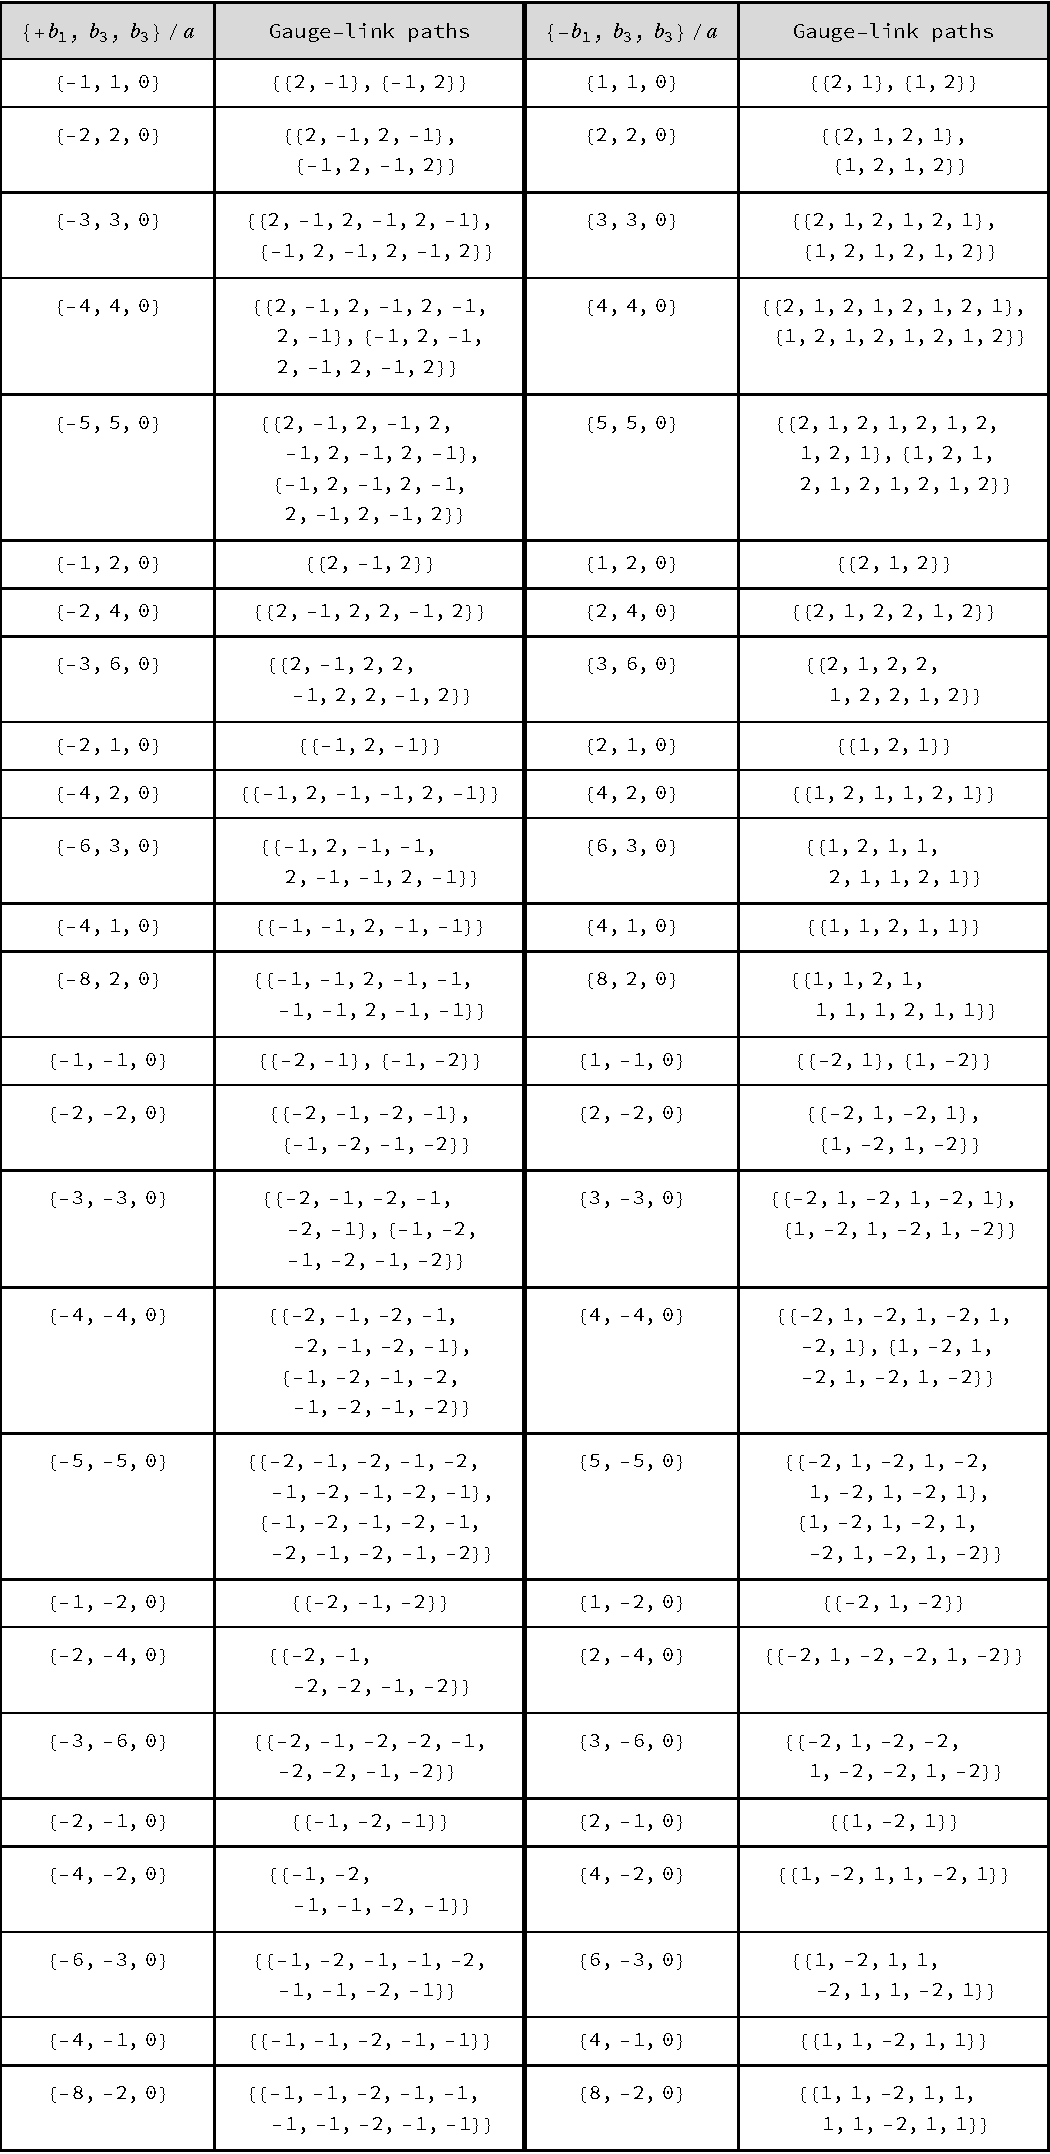
\includegraphics[width=0.8\textwidth,height=0.45\textheight,keepaspectratio]{figures/b_gauge_links_for_table3.pdf}
        \caption{Mirrored gauge link sequences for $-b_1$ (negative longitudinal separation).Symmetric sets of step-wise gauge link paths required to access finite $\pm b \cdot P$ and isolate the real and imaginary components of the invariant amplitudes. Our lattice size is $\{\hat{L}^3\times\hat{T}\}=\{32^3\times96\}$ and the lattice spacing is $a=0.11403\text{ fm}$.}
        \label{tab:b_table_neg_b1}
\end{table*}
\subsubsection{Symmetry Improving Operation (Path Averaging) for $\vect{b}$}
\label{sec:b_path_averaging}

Several quark separation vectors $\vect{b}$ have the same path degeneracy as the staple direction vector $\vect{v}$ (Sec.~\ref{sec:spatial_interpolation}). We treat it the same way: we average the correlation function over all equivalent step-wise paths that share the same origin and endpoint, as illustrated for a single coordinate in Figure \ref{fig:b_path_example}. 

\begin{figure}[htpb]
    \centering
    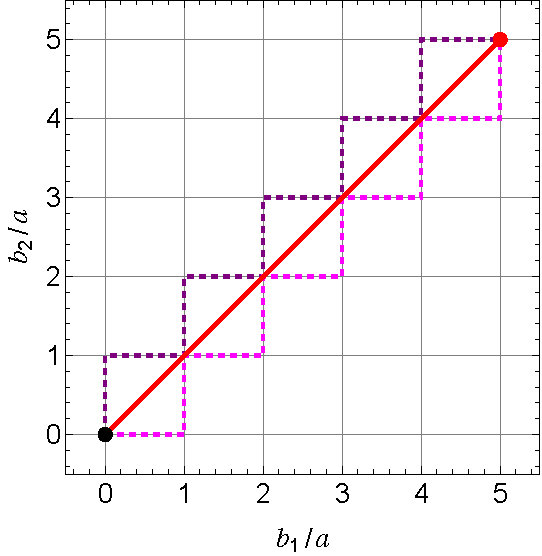
\includegraphics[width=0.3\linewidth]{figures/Example_b_plot_with_2path.pdf}
    \caption{Illustration of path degeneracy for the quark separation vector $\vect{b}$. Distinct step-wise permutations (solid and dashed lines) terminating at the same Cartesian coordinate are averaged to suppress local gauge noise.}
    \label{fig:b_path_example}
\end{figure}
Applying this symmetry-improving operation (path-averaging) strategy across the entire target grid yields the full network of smoothed off-axis trajectories, visualized in Figure \ref{fig:b_full_network}.

\begin{figure}[htpb]
    \centering
    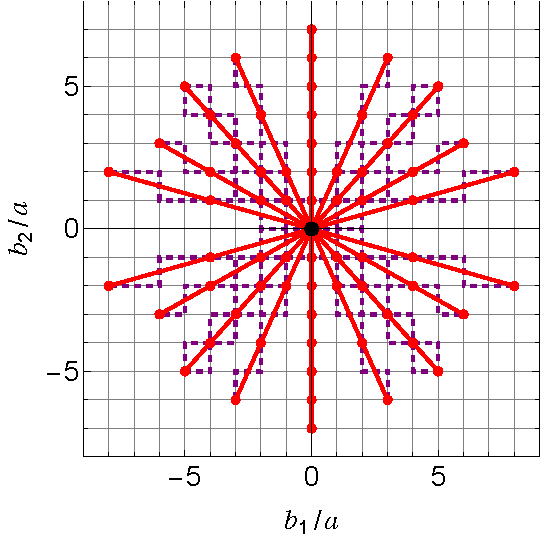
\includegraphics[width=0.4\linewidth]{figures/bL_bT_plot_with_path.pdf}
    \caption{The full network of path-averaged $\vect{b}$ vectors in the $b_1/a - b_2/a$ plane. Solid red lines represent the ideal vectors, while dashed lines illustrate the underlying degenerate staircase paths calculated and averaged on the discrete lattice.}
    \label{fig:b_full_network}
\end{figure}

\begin{widetext}
\section{Solving for the amplitudes}
\label{app:solve}
To extract the physical Sivers shift from the lattice, we must isolate the specific invariant amplitudes $\tAmp_{2B}$ and $\tAmp_{12B}$ from the raw correlator data. We start from the parametrization of the unsubtracted correlator in Eq.~\eqref{eq-phitildedecomp}~\cite{Musch:2011er}. While this parametrization describes a continuous gauge link extending to infinity, we adopt an equivalent representation for lattice calculations in which the structures depend explicitly on the finite staple extent $\eta$. This form remains well defined even in the $v \cdot P = 0$ limit. We obtain it by making the substitution $v \rightarrow \eta v$ and extracting the scaling factors $(v \tcdot P)^{-n}$ as discussed in Appendix~\ref{app:symmetries}:
 \begin{align}
    \frac{1}{2}\widetilde \Phi^{[\gamma^\mu]}_{\unsub}=\frac{1}{2} R_{\gamma^{\mu}} E_N & =  
		P^\mu\, \tilde a_2 - i \mN^2 \bvec^\mu\, \tilde a_3
		- i \mN \epsilon^{\mu \nu \alpha \beta} P_\nu \bvec_\alpha S_\beta\, \tilde a_{12} \nonumber \\ &
		~~+ \mN^2 \eta v^\mu\, \tilde b_1 
		+ \mN \epsilon^{\mu \nu \alpha \beta} P_\nu \eta v_\alpha S_\beta\, \tilde b_7  
		-  i \mN^3 \epsilon^{\mu \nu \alpha \beta} \bvec_\nu \eta v_\alpha S_\beta\, \tilde b_8 \nonumber \\ &
		~~- \mN^3 (\bvec \tcdot S) \epsilon^{\mu \nu \alpha \beta} P_\nu \bvec_\alpha \eta v_\beta\, \tilde b_9
		-i \mN^3 (v \tcdot S) \epsilon^{\mu \nu \alpha \beta} P_\nu \bvec_\alpha \eta^2 v_\beta \tilde b_{10}
\end{align}
To evaluate Eq.~\eqref{eq-phitildedecomp}, we project it onto the kinematics chosen for our lattice setup. We choose a frame where the nucleon moves in the negative $\hat{1}$-direction, the spin is polarized along the $\hat{3}$-axis, and the separation and staple vectors lie in the transverse/longitudinal planes. We set $P^{\mu}=(E_N, -|\vec{P}^1|,0,0)$, $b^{\mu}=(0,b_{1},b_{2},0)$, $v^{\mu}=\pm n^{\prime}(0,v_{1},0,v_{3})$, and $S^{\mu}=(0,0,0,1)$. Throughout this derivation, $\bvec^1$ and $\bvec^2$ denote the contravariant components of $\bvec$, so that $\bvec^1=b_L$ and $\bvec^2=b_T$ in this frame. The invariant dot product is $\bvec\cdot\bvec$; it is the quantity written $\bvec^2$ in the arguments of the amplitudes $\tAmp_i(\bvec^2,\ldots)$ and is never a component. Expanding the sum over Lorentz indices for the temporal component ($\mu = 0$) and canceling the terms that vanish (such as $b^0 = 0$, $v^0 = 0$, and $\bvec \tcdot S = 0$), we find %for each $\gamma^{\mu}$:
\begin{align}
    \frac{1}{2}\widetilde \Phi^{[\gamma^{0}]}_{\unsub} & = 
		P^0\, \tAmp_2 - \cancelto{0}{i \mN^2 \bvec^0\, \tAmp_3}
		- i \mN \underbrace{\epsilon^{0 123}}_{1} |\vec{P}^1| \bvec_2 S_3\, \tAmp_{12} \nonumber \\ &
		~~+ \cancelto{0}{\frac{\mN^2}{(v \tcdot P)} v^0\, \tBmp_1 }
		+ \cancelto{0}{\frac{\mN}{v \tcdot P} \epsilon^{0 113} P_1 v_1 S_3\, \tBmp_7  }+ \cancelto{0}{\frac{\mN}{v \tcdot P} \epsilon^{0 133} P_1 v_3 S_3\, \tBmp_7  }
		 \nonumber \\ &
		~~- \frac{ i \mN^3}{v \tcdot P} \underbrace{\epsilon^{0 213}}_{-1} \bvec_2 v_1 S_3\, \tBmp_8 - \cancelto{0}{\frac{ i \mN^3}{v \tcdot P}\epsilon^{0 113} \bvec_1 v_1 S_3\, \tBmp_8}- \cancelto{0}{\frac{ i \mN^3}{v \tcdot P}\epsilon^{0 133} \bvec_1 v_3 S_3\, \tBmp_8}- \cancelto{0}{\frac{ i \mN^3}{v \tcdot P}\epsilon^{0 233} \bvec_2 v_3 S_3\, \tBmp_8}\nonumber \\ &
		~~+ \frac{\mN^3}{v \tcdot P} \cancelto{0}{(\bvec \tcdot S)} \underbrace{\epsilon^{0 123}}_{1} |\vec{P}_1| \bvec_2 v_3\, \tBmp_9- \cancelto{0}{\frac{\mN^3}{v \tcdot P} (\bvec \tcdot S) \epsilon^{0 121} P_1 \bvec_2 v_1\, \tBmp_9}- \cancelto{0}{\frac{\mN^3}{v \tcdot P} (\bvec \tcdot S) \epsilon^{0 113} P_1 \bvec_1 v_3\, \tBmp_9} \nonumber \\ &
        - \cancelto{0}{\frac{\mN^3}{v \tcdot P} (\bvec \tcdot S) \epsilon^{0 111} P_1 \bvec_1 v_1\, \tBmp_9} - \frac{i \mN^3}{(v \tcdot P)^2} (v \tcdot S) \underbrace{\epsilon^{0 123}}_{1} |\vec{P}_1| \bvec_2 v_3 \tBmp_{10}
		- \cancelto{0}{\frac{i \mN^3}{(v \tcdot P)^2} (v \tcdot S) \epsilon^{0 121} P_1 \bvec_2 v_1 \tBmp_{10}} \nonumber \\ &
        - \cancelto{0}{\frac{i \mN^3}{(v \tcdot P)^2} (v \tcdot S) \epsilon^{0 111} P_1 \bvec_1 v_1 \tBmp_{10}} - \cancelto{0}{\frac{i \mN^3}{(v \tcdot P)^2} (v \tcdot S) \epsilon^{0 113} P_1 \bvec_1 v_3 \tBmp_{10}}\\
  \Aboxed{ \frac{1}{2}\widetilde \Phi^{[\gamma^{0}]}_{\unsub}& = P^0\, \tAmp_2  - i \mN  |\vec{P}^1| \bvec_2 S_3\, \tAmp_{12}+ \frac{ i \mN^3}{v \tcdot P}  \bvec_2 v_1 S_3\, \tBmp_8- \frac{i \mN^3}{(v \tcdot P)^2} (v \tcdot S)  |P_1| \bvec_2 v_3 \tBmp_{10}}
\end{align}
Repeating this tensor contraction for the longitudinal spatial component ($\mu = 1$), taking care to track the signs of the Levi-Civita symbol, yields:
\begin{align}
    \frac{1}{2}\widetilde \Phi^{[\gamma^{1}]}_{\unsub} & = 
		-|\vec{P}^1|\, \tAmp_2 - i \mN^2 \bvec^1\, \tAmp_3
		- i \mN \underbrace{\epsilon^{1 023}}_{-1} P_0 \bvec_2 S_3\, \tAmp_{12} \nonumber \\ &
		~~+ \frac{\mN^2}{(v \tcdot P)} v^1\, \tBmp_1 
		+ \cancelto{0}{\frac{\mN}{v \tcdot P} \epsilon^{1 013} P_0 v_1 S_3\, \tBmp_7  }+ \cancelto{0}{\frac{\mN}{v \tcdot P} \epsilon^{1 033} P_0 v_3 S_3\, \tBmp_7  } \nonumber \\ &
		- \cancelto{0}{\frac{ i \mN^3}{v \tcdot P} \epsilon^{1 213} \bvec_2 v_1 S_3\, \tBmp_8}- \cancelto{0}{\frac{ i \mN^3}{v \tcdot P} \epsilon^{1 233} \bvec_2 v_3 S_3\, \tBmp_8} - \cancelto{0}{\frac{ i \mN^3}{v \tcdot P} \epsilon^{1 133} \bvec_1 v_3 S_3\, \tBmp_8}- \cancelto{0}{\frac{ i \mN^3}{v \tcdot P} \epsilon^{1 113} \bvec_1 v_1 S_3\, \tBmp_8}\nonumber \\ & 
        - \frac{\mN^3}{v \tcdot P} \cancelto{0}{(\bvec \tcdot S)} \underbrace{\epsilon^{1 023}}_{1} P_0 \bvec_2 v_3\, \tBmp_9 - \cancelto{0}{\frac{\mN^3}{v \tcdot P} (\bvec \tcdot S) \epsilon^{1 021} P_0 \bvec_2 v_1\, \tBmp_9} - \frac{i \mN^3}{(v \tcdot P)^2} (v \tcdot S) \underbrace{\epsilon^{1 023}}_{-1} P_0 \bvec_2 v_3 \tBmp_{10} \nonumber \\ & - \cancelto{0}{\frac{i \mN^3}{(v \tcdot P)^2} (v \tcdot S) \epsilon^{1 021} P_0 \bvec_2 v_1 \tBmp_{10}}\\
  \Aboxed{ \frac{1}{2}\widetilde \Phi^{[\gamma^{1}]}_{\unsub} & =-|\vec{P}^1|\, \tAmp_2+ \frac{\mN^2}{(v \tcdot P)} v^1\, \tBmp_1 
		+ i \mN  P_0 \bvec_2 S_3\, \tAmp_{12}+ \frac{i \mN^3}{(v \tcdot P)^2} (v \tcdot S)  P_0 \bvec_2 v_3 \tBmp_{10}- i \mN^2 \bvec^1\, \tAmp_3}
\end{align}
Evaluating the transverse component ($\mu=2$) isolates terms that depend on $P_0$ and the longitudinal separation $b_1$:
\begin{align}
    \frac{1}{2}\widetilde \Phi^{[\gamma^2]}_{\unsub} & = 
		 - i \mN^2 \bvec^2\, \tAmp_3
		- i \mN \underbrace{\epsilon^{2 0 1 3}}_{1} P_0 \bvec_1 S_3\, \tAmp_{12} \nonumber \\ &
		~~
		+ \frac{\mN}{v \tcdot P} \underbrace{\epsilon^{2 0 1 3}}_{1} P_0 v_1 S_3\, \tBmp_7  
		 \nonumber \\ &
		~~
		- \frac{i \mN^3}{(v \tcdot P)^2} (v \tcdot S) \underbrace{\epsilon^{2 0 1 3}}_{1} P_0 \bvec_1 v_3 \tBmp_{10}\\
  \Aboxed{\frac{1}{2}\widetilde \Phi^{[\gamma^2]}_{\unsub} & =- i \mN^2 \bvec^2\, \tAmp_3
		- i \mN  P_0 \bvec_1 S_3\, \tAmp_{12}+ \frac{\mN}{v \tcdot P}  P_0 v_1 S_3\, \tBmp_7- \frac{i \mN^3}{(v \tcdot P)^2} (v \tcdot S) P_0 \bvec_1 v_3 \tBmp_{10}}
\end{align}
Finally, the orthogonal transverse component ($\mu=3$) simplifies because of the alignment of the spin vector:
\begin{align}
    \frac{1}{2}\widetilde \Phi^{[\gamma^3]}_{\unsub} & = \frac{\mN^2}{(v \tcdot P)} v^3\, \tBmp_1 
		\nonumber \\ &
		~~
		- \frac{i \mN^3}{(v \tcdot P)^2} (v \tcdot S) \underbrace{\epsilon^{3 0 2 1}}_{1} P_0 \bvec_2 v_1 \tBmp_{10}\\
  \Aboxed{\frac{1}{2}\widetilde \Phi^{[\gamma^3]}_{\unsub}& = \frac{\mN^2}{(v \tcdot P)} v^3\, \tBmp_1- \frac{i \mN^3}{(v \tcdot P)^2} (v \tcdot S)  P_0 \bvec_2 v_1 \tBmp_{10}}
\end{align}
Collecting these boxed results gives the full system of equations mapping the infinite-link continuous amplitudes to the projected correlator components:
\begin{align}
   \Aboxed{ \frac{1}{2}\widetilde \Phi^{[\gamma^{0}]}_{\unsub}& = P^0\, \tAmp_2  - i \mN  |\vec{P}^1| \bvec_2 S_3\, \tAmp_{12}+ \frac{ i \mN^3}{v \tcdot P}  \bvec_2 v_1 S_3\, \tBmp_8- \frac{i \mN^3}{(v \tcdot P)^2} (v \tcdot S)  |P_1| \bvec_2 v_3 \tBmp_{10}}\\
   \Aboxed{ \frac{1}{2}\widetilde \Phi^{[\gamma^{1}]}_{\unsub} & =-|\vec{P}^1|\, \tAmp_2- i \mN^2 \bvec^1\, \tAmp_3+ \frac{\mN^2}{(v \tcdot P)} v^1\, \tBmp_1 
		+ i \mN  P_0 \bvec_2 S_3\, \tAmp_{12}+ \frac{i \mN^3}{(v \tcdot P)^2} (v \tcdot S)  P_0 \bvec_2 v_3 \tBmp_{10}}\\
   \Aboxed{\frac{1}{2}\widetilde \Phi^{[\gamma^2]}_{\unsub} & =- i \mN^2 \bvec^2\, \tAmp_3
		- i \mN  P_0 \bvec_1 S_3\, \tAmp_{12}+ \frac{\mN}{v \tcdot P}  P_0 v_1 S_3\, \tBmp_7- \frac{i \mN^3}{(v \tcdot P)^2} (v \tcdot S) P_0 \bvec_1 v_3 \tBmp_{10}}\\
    \Aboxed{\frac{1}{2}\widetilde \Phi^{[\gamma^3]}_{\unsub}& = \frac{\mN^2}{(v \tcdot P)} v^3\, \tBmp_1- \frac{i \mN^3}{(v \tcdot P)^2} (v \tcdot S)  P_0 \bvec_2 v_1 \tBmp_{10}}
\end{align}
We structure this system as a column vector to streamline the upcoming algebraic inversions:
\begin{align}
    \begin{pmatrix}
        \rule{0pt}{16pt} \widetilde \Phi^{[\gamma^{0}]}_{\unsub}\\
        \rule{0pt}{16pt} \widetilde \Phi^{[\gamma^{1}]}_{\unsub}\\
        \rule{0pt}{16pt} \widetilde \Phi^{[\gamma^{2}]}_{\unsub}\\
        \rule{0pt}{16pt} \widetilde \Phi^{[\gamma^{3}]}_{\unsub}
    \end{pmatrix} &=2\begin{pmatrix}
       \rule{0pt}{16pt}  P^0\, \tAmp_2  - i \mN  |\vec{P}^1| \bvec_2 S_3\, \tAmp_{12}+ \frac{ i \mN^3}{v \tcdot P}  \bvec_2 v_1 S_3\, \tBmp_8- \frac{i \mN^3}{(v \tcdot P)^2} (v \tcdot S)  |P_1| \bvec_2 v_3 \tBmp_{10}\\
        \rule{0pt}{16pt} -|\vec{P}^1|\, \tAmp_2- i \mN^2 \bvec^1\, \tAmp_3+ \frac{\mN^2}{(v \tcdot P)} v^1\, \tBmp_1 
		+ i \mN  P_0 \bvec_2 S_3\, \tAmp_{12}+ \frac{i \mN^3}{(v \tcdot P)^2} (v \tcdot S)  P_0 \bvec_2 v_3 \tBmp_{10}\\
         \rule{0pt}{16pt} - i \mN^2 \bvec^2\, \tAmp_3
		- i \mN  P_0 \bvec_1 S_3\, \tAmp_{12}+ \frac{\mN}{v \tcdot P}  P_0 v_1 S_3\, \tBmp_7- \frac{i \mN^3}{(v \tcdot P)^2} (v \tcdot S) P_0 \bvec_1 v_3 \tBmp_{10}\\
        \rule{0pt}{16pt} \frac{\mN^2}{(v \tcdot P)} v^3\, \tBmp_1- \frac{i \mN^3}{(v \tcdot P)^2} (v \tcdot S)  P_0 \bvec_2 v_1 \tBmp_{10}
    \end{pmatrix}
\end{align}
To match standard contravariant Lorentz notation, we raise the spatial indices using the Minkowski metric $g^{\mu\nu} = \text{diag}(1, -1, -1, -1)$. This introduces a relative minus sign for the spatial components (e.g., $P_1 = -P^1$, $b_2 = -b^2$):
\begin{align}
    \begin{pmatrix}
        \rule{0pt}{16pt} \widetilde \Phi^{[\gamma^{0}]}_{\unsub}\\
        \rule{0pt}{16pt} \widetilde \Phi^{[\gamma^{1}]}_{\unsub}\\
        \rule{0pt}{16pt} \widetilde \Phi^{[\gamma^{2}]}_{\unsub}\\
        \rule{0pt}{16pt} \widetilde \Phi^{[\gamma^{3}]}_{\unsub}
    \end{pmatrix} &=2\begin{pmatrix}
       \rule{0pt}{16pt}  P^0\, \tAmp_2  - i \mN  |\vec{P}^1| \bvec^2 S^3\, \tAmp_{12}- \frac{ i \mN^3}{v \tcdot P}  \bvec^2 v^1 S^3\, \tBmp_8- \frac{i \mN^3}{(v \tcdot P)^2} (v \tcdot S)  |\vec{P}^1| \bvec^2 v^3 \tBmp_{10}\\
        \rule{0pt}{16pt} -|\vec{P}^1|\, \tAmp_2- i \mN^2 \bvec^1\, \tAmp_3+ \frac{\mN^2}{(v \tcdot P)} v^1\, \tBmp_1 
		+ i \mN  P^0 \bvec^2 S^3\, \tAmp_{12}+ \frac{i \mN^3}{(v \tcdot P)^2} (v \tcdot S)  P^0 \bvec^2 v^3 \tBmp_{10}\\
         \rule{0pt}{16pt} - i \mN^2 \bvec^2\, \tAmp_3
		- i \mN  P^0 \bvec^1 S^3\, \tAmp_{12}+ \frac{\mN}{v \tcdot P}  P^0 v^1 S^3\, \tBmp_7- \frac{i \mN^3}{(v \tcdot P)^2} (v \tcdot S) P^0 \bvec^1 v^3 \tBmp_{10}\\
        \rule{0pt}{16pt} \frac{\mN^2}{(v \tcdot P)} v^3\, \tBmp_1- \frac{i \mN^3}{(v \tcdot P)^2} (v \tcdot S)  P^0 \bvec^2 v^1 \tBmp_{10}
    \end{pmatrix}
\end{align}
To connect these continuous amplitudes to the discretized finite-link observables simulated on the lattice, we use the mapping of Eq.~\eqref{eq-ab} between the infinite-link amplitudes ($\tAmp_i$, $\tBmp_i$) and the finite-link amplitudes ($\tilde{a}_i$, $\tilde{b}_i$). The finite-link amplitudes are complex-valued functions, which we decompose into their real and imaginary components:
\begin{align}
    \tilde{a}_i&=\tilde{a}^{\text{Re}}_i+i\tilde{a}^{\text{Im}}_i\\
    \tilde{b}_i&=\tilde{b}^{\text{Re}}_i+i\tilde{b}^{\text{Im}}_i
\end{align}
The lattice evaluation also requires converting the continuous Minkowski gamma matrices ($\gamma_M$) into the Euclidean conventions ($\gamma_E$) used by the lattice simulation software:
\begin{itemize}
    \item Correct Euclidean $\longleftrightarrow$ Minkowski $\gamma$-matrices notation:
    \begin{align}
        \Aboxed{\gamma^{1}_{E}=&+i\gamma^{1}_{M}}\\
        \Aboxed{\gamma^{2}_{E}=&-i\gamma^{2}_{M}}\\
        \Aboxed{\gamma^{3}_{E}=&+i\gamma^{3}_{M}}\\
        \Aboxed{\gamma^{4}_{E}=&\gamma^{0}_{M}}\\
        \boxed{\gamma^{5}_{E}}=&\gamma^{1}_{E}\gamma^{2}_{E}\gamma^{3}_{E}\gamma^{4}_{E}=\boxed{-\gamma^{5}_{M}}=-i\gamma^{0}_{M}\gamma^{1}_{M}\gamma^{2}_{M}\gamma^{3}_{M}
    \end{align}
\end{itemize}
Substituting the Euclidean gamma structures and mapping $P^0 \to E_N$, we rewrite the column vector entirely in terms of the lattice ratio observables $R_{\Gamma(i)}$ and the finite-link amplitudes. The index $i \in \{1,2,4,8\}$ labels each Dirac structure by its bit-encoded position (CHROMA and QLUA convention) in our operator basis, matching the correspondence $\Gamma(1)=[+i\gamma^1]$, $\Gamma(2)=[-i\gamma^2]$, $\Gamma(4)=[+i\gamma^3]$, and $\Gamma(8)=[\gamma^0]$ used below:
\begin{align}
    \begin{pmatrix}
        \rule{0pt}{16pt} R_{\Gamma(1)}\\
        \rule{0pt}{16pt} R_{\Gamma(2)}\\
        \rule{0pt}{16pt} R_{\Gamma(4)}\\
        \rule{0pt}{16pt} R_{\Gamma(8)}
    \end{pmatrix} = \begin{pmatrix}
        \rule{0pt}{16pt} R_{[+i\gamma^1]}\\
        \rule{0pt}{16pt} R_{[-i\gamma^2]}\\
        \rule{0pt}{16pt} R_{[+i\gamma^3]}\\
        \rule{0pt}{16pt} R_{[\gamma^0]}
    \end{pmatrix} &=2\begin{pmatrix}
        \rule{0pt}{16pt} -i\frac{|\vec{P}^1|}{E_N}\, \tilde a_2+  \frac{\mN^2}{E_N} \bvec^1\, \tilde a_3+ i\frac{\mN^2}{E_N} \eta v^1\, \tilde b_1 
		-  \mN  \bvec^2 \, \tilde a_{12}+  \mN^3  \bvec^2 \eta^2 (v^3)^2 \tilde b_{10}\\
         \rule{0pt}{16pt} -  \frac{\mN^2}{E_N} \bvec^2\, \tilde a_3
		-  \mN   \bvec^1  \tilde a_{12}-i \mN \eta  v^1  \tilde b_7+ \mN^3  \bvec^1 \eta^2 (v^3)^2 \tilde b_{10}\\
        \rule{0pt}{16pt} i\frac{\mN^2}{E_N} \eta v^3\, \tilde b_1-  \mN^3 \bvec^2 \eta^2 v^1 v^3\tilde b_{10}\\
         \rule{0pt}{16pt}   \tilde a_2  - i \mN  \frac{|\vec{P}^1|}{E_N} \bvec^2  \tilde a_{12}- \frac{ i \mN^3}{E_N}  \bvec^2 \eta v^1  \tilde b_8+ \frac{i \mN^3}{E_N}  |\vec{P}^1| \bvec^2 \eta^2 (v^3)^2 \tilde b_{10}
    \end{pmatrix}
\end{align}
To separate the real and imaginary amplitude contributions analytically, we split this matrix equation into two sets by flipping the longitudinal separation component $b^1$. For a strictly positive longitudinal separation ($+b^1$), writing out the real and imaginary parts of the correlator ratios gives:
\begin{align}
    \begin{pmatrix}
        \rule{0pt}{16pt} \text{Re}\{ R_{\Gamma(1)}\}^{[+b^1]} \\
        \rule{0pt}{16pt} \text{Im}\{ R_{\Gamma(1)}\}^{[+b^1]} \\
        \rule{0pt}{16pt} \text{Re}\{ R_{\Gamma(2)}\}^{[+b^1]} \\
        \rule{0pt}{16pt} \text{Im}\{ R_{\Gamma(2)}\}^{[+b^1]} \\
        \rule{0pt}{16pt} \text{Re}\{ R_{\Gamma(4)}\}^{[+b^1]} \\
        \rule{0pt}{16pt} \text{Im}\{ R_{\Gamma(4)}\}^{[+b^1]} \\
        \rule{0pt}{16pt} \text{Re}\{ R_{\Gamma(8)}\}^{[+b^1]} \\
        \rule{0pt}{16pt} \text{Im}\{ R_{\Gamma(8)}\}^{[+b^1]}
    \end{pmatrix} &= 2\begin{pmatrix}
     \rule{0pt}{16pt}   \frac{\mN^2}{E_N} \bvec^1\, \tilde a^{\text{Re}}_3-  \mN  \bvec^2 \, \tilde a^{\text{Re}}_{12}+  \mN^3  \bvec^2 \eta^2 (v^3)^2 \tilde b^{\text{Re}}_{10} +\frac{|\vec{P}^1|}{E_N}\, \tilde a^{\text{Im}}_2- \frac{\mN^2}{E_N} \eta v^1\, \tilde b^{\text{Im}}_1\\
      \rule{0pt}{16pt}  -\frac{|\vec{P}^1|}{E_N}\, \tilde a^{\text{Re}}_2+ \frac{\mN^2}{E_N} \eta v^1\, \tilde b^{\text{Re}}_1 + \frac{\mN^2}{E_N} \bvec^1\, \tilde a^{\text{Im}}_3-  \mN  \bvec^2 \, \tilde a^{\text{Im}}_{12}+  \mN^3  \bvec^2 \eta^2 (v^3)^2 \tilde b^{\text{Im}}_{10}\\
      \rule{0pt}{16pt}  -  \frac{\mN^2}{E_N} \bvec^2\, \tilde a^{\text{Re}}_3
		-  \mN   \bvec^1  \tilde a^{\text{Re}}_{12}+ \mN^3  \bvec^1 \eta^2 (v^3)^2 \tilde b^{\text{Re}}_{10}+\mN \eta v^1  \tilde b^{\text{Im}}_7 \\
      \rule{0pt}{16pt} - \mN \eta v^1  \tilde b^{\text{Re}}_7 -  \frac{\mN^2}{E_N} \bvec^2\, \tilde a^{\text{Im}}_3
		-  \mN   \bvec^1  \tilde a^{\text{Im}}_{12}+ \mN^3  \bvec^1 \eta^2 (v^3)^2 \tilde b^{\text{Im}}_{10}\\
      \rule{0pt}{16pt} -\mN^3 \bvec^2 \eta^2 v^1 v^3\tilde b^{\text{Re}}_{10}-\frac{\mN^2}{E_N} \eta v^3\, \tilde b^{\text{Im}}_1\\
      \rule{0pt}{16pt} \frac{\mN^2}{E_N} \eta v^3\, \tilde b^{\text{Re}}_1 -\mN^3 \bvec^2 \eta^2 v^1 v^3\tilde b^{\text{Im}}_{10}\\
      \rule{0pt}{16pt}  \tilde a^{\text{Re}}_2 +  \mN  \frac{|\vec{P}^1|}{E_N} \bvec^2  \tilde a^{\text{Im}}_{12}+ \frac{  \mN^3}{E_N}  \bvec^2 \eta v^1  \tilde b^{\text{Im}}_8- \frac{ \mN^3}{E_N}  |\vec{P}^1| \bvec^2 \eta^2 (v^3)^2 \tilde b^{\text{Im}}_{10}\\
      \rule{0pt}{16pt} -  \mN  \frac{|\vec{P}^1|}{E_N} \bvec^2  \tilde a^{\text{Re}}_{12}- \frac{  \mN^3}{E_N}  \bvec^2 \eta v^1  \tilde b^{\text{Re}}_8+ \frac{ \mN^3}{E_N}  |\vec{P}^1| \bvec^2 \eta^2 (v^3)^2 \tilde b^{\text{Re}}_{10}+\tilde a^{\text{Im}}_2
    \end{pmatrix}
\end{align}
Evaluating the system for the negated separation ($-b^1$) flips the signs of selected terms according to the parity constraints of Eq.~\eqref{eq-ReIm-parity}. By construction, the imaginary parts of the amplitudes are odd functions of $b^1$ ($\tAmp_i^{\text{Im}}=\tAmp_i^{\text{(b-odd)}}=\tAmp_i^{\text{($b^1$-odd)}}$ and  $\tBmp_i^{\text{Im}}=\tBmp_i^{\text{(b-odd)}}=\tBmp_i^{\text{($b^1$-odd)}}$). Applying these parity reversals yields the conjugate matrix:
\begin{align}
    \begin{pmatrix}
        \rule{0pt}{16pt} \text{Re}\{ R_{\Gamma(1)}\}^{[-b^1]} \\
        \rule{0pt}{16pt} \text{Im}\{ R_{\Gamma(1)}\}^{[-b^1]} \\
        \rule{0pt}{16pt} \text{Re}\{ R_{\Gamma(2)}\}^{[-b^1]} \\
        \rule{0pt}{16pt} \text{Im}\{ R_{\Gamma(2)}\}^{[-b^1]} \\
        \rule{0pt}{16pt} \text{Re}\{ R_{\Gamma(4)}\}^{[-b^1]} \\
        \rule{0pt}{16pt} \text{Im}\{ R_{\Gamma(4)}\}^{[-b^1]} \\
        \rule{0pt}{16pt} \text{Re}\{ R_{\Gamma(8)}\}^{[-b^1]} \\
        \rule{0pt}{16pt} \text{Im}\{ R_{\Gamma(8)}\}^{[-b^1]}
    \end{pmatrix} &= 2\begin{pmatrix}
     \rule{0pt}{16pt}   \textcolor{red}{-}\frac{\mN^2}{E_N} \bvec^1\, \tilde a^{\text{Re}}_3-  \mN  \bvec^2 \, \tilde a^{\text{Re}}_{12}+  \mN^3  \bvec^2 \eta^2 (v^3)^2 \tilde b^{\text{Re}}_{10} \textcolor{red}{-}\frac{|\vec{P}^1|}{E_N}\, \tilde a^{\text{Im}}_2\textcolor{red}{+} \frac{\mN^2}{E_N} \eta v^1\, \tilde b^{\text{Im}}_1\\
      \rule{0pt}{16pt}  -\frac{|\vec{P}^1|}{E_N}\, \tilde a^{\text{Re}}_2+ \frac{\mN^2}{E_N} \eta v^1\, \tilde b^{\text{Re}}_1 + \frac{\mN^2}{E_N} \bvec^1\, \tilde a^{\text{Im}}_3\textcolor{red}{+} \mN  \bvec^2 \, \tilde a^{\text{Im}}_{12}\textcolor{red}{-} \mN^3  \bvec^2 \eta^2 (v^3)^2 \tilde b^{\text{Im}}_{10}\\
      \rule{0pt}{16pt}  - \frac{\mN^2}{E_N} \bvec^2\, \tilde a^{\text{Re}}_3
		\textcolor{red}{+}  \mN   \bvec^1  \tilde a^{\text{Re}}_{12}\textcolor{red}{-} \mN^3  \bvec^1 \eta^2 (v^3)^2 \tilde b^{\text{Re}}_{10}\textcolor{red}{-}\mN \eta v^1  \tilde b^{\text{Im}}_7 \\
      \rule{0pt}{16pt} - \mN \eta v^1  \tilde b^{\text{Re}}_7 \textcolor{red}{+}  \frac{\mN^2}{E_N} \bvec^2\, \tilde a^{\text{Im}}_3
		- \mN   \bvec^1  \tilde a^{\text{Im}}_{12} +\mN^3  \bvec^1 \eta^2 (v^3)^2 \tilde b^{\text{Im}}_{10}\\
      \rule{0pt}{16pt}-\mN^3 \bvec^2 \eta^2 v^1 v^3\tilde b^{\text{Re}}_{10}\textcolor{red}{+}\frac{\mN^2}{E_N} \eta v^3\, \tilde b^{\text{Im}}_1\\
      \rule{0pt}{16pt} \frac{\mN^2}{E_N} \eta v^3\, \tilde b^{\text{Re}}_1 \textcolor{red}{+} \mN^3 \bvec^2 \eta^2 v^1 v^3\tilde b^{\text{Im}}_{10}\\
      \rule{0pt}{16pt}  \tilde a^{\text{Re}}_2 \textcolor{red}{-}  \mN  \frac{|\vec{P}^1|}{E_N} \bvec^2  \tilde a^{\text{Im}}_{12}\textcolor{red}{-} \frac{  \mN^3}{E_N}  \bvec^2 \eta v^1  \tilde b^{\text{Im}}_8\textcolor{red}{+} \frac{ \mN^3}{E_N}  |\vec{P}^1| \bvec^2 \eta^2 (v^3)^2 \tilde b^{\text{Im}}_{10}\\
      \rule{0pt}{16pt} - \mN  \frac{|\vec{P}^1|}{E_N} \bvec^2  \tilde a^{\text{Re}}_{12}- \frac{  \mN^3}{E_N}  \bvec^2 \eta v^1  \tilde b^{\text{Re}}_8 + \frac{ \mN^3}{E_N}  |\vec{P}^1| \bvec^2 \eta^2 (v^3)^2 \tilde b^{\text{Re}}_{10}\textcolor{red}{-}\tilde a^{\text{Im}}_2
    \end{pmatrix}
\end{align}
By taking the symmetric average of the two matrices, $\frac{1}{2}\left(R^{[+b]} + R^{[-b]}\right)$, we project out the $b$-even combination, isolating the real parts of the requisite amplitudes:
\begin{align}
    \begin{pmatrix}
        \rule{0pt}{16pt} \text{Re}\{ R_{\Gamma(1)}\}^{[b^{1}\text{-even}]} \\
        \rule{0pt}{16pt} \text{Im}\{ R_{\Gamma(1)}\}^{[b^{1}\text{-even}]} \\
        \rule{0pt}{16pt} \text{Re}\{ R_{\Gamma(2)}\}^{[b^{1}\text{-even}]} \\
        \rule{0pt}{16pt} \text{Im}\{ R_{\Gamma(2)}\}^{[b^{1}\text{-even}]} \\
        \rule{0pt}{16pt} \text{Re}\{ R_{\Gamma(4)}\}^{[b^{1}\text{-even}]} \\
        \rule{0pt}{16pt} \text{Im}\{ R_{\Gamma(4)}\}^{[b^{1}\text{-even}]} \\
        \rule{0pt}{16pt} \text{Re}\{ R_{\Gamma(8)}\}^{[b^{1}\text{-even}]} \\
        \rule{0pt}{16pt} \text{Im}\{ R_{\Gamma(8)}\}^{[b^{1}\text{-even}]}
    \end{pmatrix} &= 2\begin{pmatrix}
     \rule{0pt}{16pt}  -  \mN  \bvec^2 \, \tilde a^{\text{Re}}_{12}+  \mN^3  \bvec^2 \eta^2 (v^3)^2 \tilde b^{\text{Re}}_{10} \\
      \rule{0pt}{16pt}  -\frac{|\vec{P}^1|}{E_N}\, \tilde a^{\text{Re}}_2+ \frac{\mN^2}{E_N} \eta v^1\, \tilde b^{\text{Re}}_1 + \frac{\mN^2}{E_N} \bvec^1\, \tilde a^{\text{Im}}_3\\
      \rule{0pt}{16pt}  -  \frac{\mN^2}{E_N} \bvec^2\, \tilde a^{\text{Re}}_3
		\\
      \rule{0pt}{16pt} - \mN \eta v^1  \tilde b^{\text{Re}}_7
		-  \mN   \bvec^1  \tilde a^{\text{Im}}_{12}+ \mN^3  \bvec^1 \eta^2 (v^3)^2 \tilde b^{\text{Im}}_{10}\\
      \rule{0pt}{16pt} -\mN^3 \bvec^2 \eta^2 v^1 v^3\tilde b^{\text{Re}}_{10}\\
      \rule{0pt}{16pt} \frac{\mN^2}{E_N} \eta v^3\, \tilde b^{\text{Re}}_1 \\
      \rule{0pt}{16pt}  \tilde a^{\text{Re}}_2\\
      \rule{0pt}{16pt} -  \mN  \frac{|\vec{P}^1|}{E_N} \bvec^2  \tilde a^{\text{Re}}_{12}- \frac{  \mN^3}{E_N}  \bvec^2 \eta v^1  \tilde b^{\text{Re}}_8+ \frac{ \mN^3}{E_N}  |\vec{P}^1| \bvec^2 \eta^2 (v^3)^2 \tilde b^{\text{Re}}_{10}
    \end{pmatrix}
\end{align}
Conversely, taking the antisymmetric half-difference of the two matrices, $\frac{1}{2}\left(R^{[+b]} - R^{[-b]}\right)$, projects out the $b$-odd combination, isolating the imaginary parts:
\begin{align}
    \begin{pmatrix}
        \rule{0pt}{16pt} \text{Re}\{ R_{\Gamma(1)}\}^{[b^{1}\text{-odd}]} \\
        \rule{0pt}{16pt} \text{Im}\{ R_{\Gamma(1)}\}^{[b^{1}\text{-odd}]} \\
        \rule{0pt}{16pt} \text{Re}\{ R_{\Gamma(2)}\}^{[b^{1}\text{-odd}]} \\
        \rule{0pt}{16pt} \text{Im}\{ R_{\Gamma(2)}\}^{[b^{1}\text{-odd}]} \\
        \rule{0pt}{16pt} \text{Re}\{ R_{\Gamma(4)}\}^{[b^{1}\text{-odd}]} \\
        \rule{0pt}{16pt} \text{Im}\{ R_{\Gamma(4)}\}^{[b^{1}\text{-odd}]} \\
        \rule{0pt}{16pt} \text{Re}\{ R_{\Gamma(8)}\}^{[b^{1}\text{-odd}]} \\
        \rule{0pt}{16pt} \text{Im}\{ R_{\Gamma(8)}\}^{[b^{1}\text{-odd}]}
    \end{pmatrix} &= 2\begin{pmatrix}
     \rule{0pt}{16pt}   \frac{\mN^2}{E_N} \bvec^1\, \tilde a^{\text{Re}}_3+\frac{|\vec{P}^1|}{E_N}\, \tilde a^{\text{Im}}_2- \frac{\mN^2}{E_N} \eta v^1\, \tilde b^{\text{Im}}_1\\
      \rule{0pt}{16pt}  -  \mN  \bvec^2 \, \tilde a^{\text{Im}}_{12}+  \mN^3  \bvec^2 \eta^2 (v^3)^2 \tilde b^{\text{Im}}_{10}\\
      \rule{0pt}{16pt}  
		-  \mN   \bvec^1  \tilde a^{\text{Re}}_{12}+ \mN^3  \bvec^1 \eta^2 (v^3)^2 \tilde b^{\text{Re}}_{10}+\mN \eta v^1  \tilde b^{\text{Im}}_7 \\
      \rule{0pt}{16pt}  -  \frac{\mN^2}{E_N} \bvec^2\, \tilde a^{\text{Im}}_3\\
      \rule{0pt}{16pt} -\frac{\mN^2}{E_N} \eta v^3\, \tilde b^{\text{Im}}_1\\
      \rule{0pt}{16pt}  -\mN^3 \bvec^2 \eta^2 v^1 v^3\tilde b^{\text{Im}}_{10}\\
      \rule{0pt}{16pt}    \mN  \frac{|\vec{P}^1|}{E_N} \bvec^2  \tilde a^{\text{Im}}_{12}+ \frac{  \mN^3}{E_N}  \bvec^2 \eta v^1  \tilde b^{\text{Im}}_8- \frac{ \mN^3}{E_N}  |\vec{P}^1| \bvec^2 \eta^2 (v^3)^2 \tilde b^{\text{Im}}_{10}\\
      \rule{0pt}{16pt} \tilde a^{\text{Im}}_2
    \end{pmatrix}
\end{align}
To analytically reconstruct the Sivers shift, we solve these projected systems for the amplitudes that drive the Sivers effect: $\tilde a_2$, $\tilde b_1$, $\tilde a_{12}$, and $\tilde b_8$. Reading directly from the $b$-even system, we isolate the real components:
\begin{align}
    \tilde a^{\text{Re}}_2 = & \frac{1}{2}\text{Re}\{ R_{\Gamma(8)}\}^{[b^{1}\text{-even}]} \\
    \tilde b^{\text{Re}}_1 = & \frac{E_{N}}{2\mN^2 \eta v^3} \text{Im}\{ R_{\Gamma(4)}\}^{[b^{1}\text{-even}]}
\end{align}
Substituting the appropriate matrix rows, we decouple $\tilde a_{12}$ and $\tilde b_8$:
\begin{align}
   \tilde a^{\text{Re}}_{12}=&\frac{-1}{2\mN  \bvec^2}\left[\text{Re}\{ R_{\Gamma(1)}\}^{[b^{1}\text{-even}]}+\frac{v^3}{v^1}\text{Re}\{ R_{\Gamma(4)}\}^{[b^{1}\text{-even}]}\right]
\end{align}
\begin{align}
    \tilde b^{\text{Re}}_8=&\frac{-E_N}{ 2\mN^3 \bvec^2 \eta v^1 }\left[\text{Im}\{ R_{\Gamma(8)}\}^{[b^{1}\text{-even}]}+\frac{|\vec{P}^1|v^3}{E_N v^1}\text{Re}\{ R_{\Gamma(4)}\}^{[b^{1}\text{-even}]}+ 2\mN  \frac{|\vec{P}^1|}{E_N} \bvec^2  \tilde a^{\text{Re}}_{12}\right]
\end{align}
Applying identical algebraic decoupling to the $b$-odd system, we isolate the corresponding imaginary components:
\begin{align}
    \tilde a^{\text{Im}}_2 = & \frac{1}{2}\text{Im}\{ R_{\Gamma(8)}\}^{[b^{1}\text{-odd}]} \\
    \tilde b^{\text{Im}}_1 = & \frac{-E_{N}}{2\mN^2 \eta v^3} \text{Re}\{ R_{\Gamma(4)}\}^{[b^{1}\text{-odd}]}
\end{align}
and the remaining transverse amplitudes:
\begin{align}
   \tilde a^{\text{Im}}_{12}=&\frac{-1}{2\mN  \bvec^2}\left[\text{Im}\{ R_{\Gamma(1)}\}^{[b^{1}\text{-odd}]}+\frac{v^3}{v^1}\text{Im}\{ R_{\Gamma(4)}\}^{[b^{1}\text{-odd}]}\right]
\end{align}
\begin{align}
    \tilde b^{\text{Im}}_8=&\frac{E_N}{ 2\mN^3 \bvec^2 \eta v^1 }\left[\text{Re}\{ R_{\Gamma(8)}\}^{[b^{1}\text{-odd}]}-\frac{|\vec{P}^1|v^3}{E_N v^1}\text{Im}\{ R_{\Gamma(4)}\}^{[b^{1}\text{-odd}]}- 2\mN  \frac{|\vec{P}^1|}{E_N} \bvec^2  \tilde a^{\text{Im}}_{12}\right]
\end{align}
Finally, we convert these finite-link evaluations ($\tilde a_i, \tilde b_i$) back into the standard continuum-invariant amplitudes ($\tAmp_i, \tBmp_i$) using the proportionality dictionary:
\begin{align}
	\tAmp_i & = \tilde a_i \\
	 \tBmp_i & = (\eta v \tcdot P)^n\ \tilde b_i
\end{align}
\end{widetext}
